%%%%%%%%%%%%%%%%%%%%%%%%%%%%%%%%%%%%%%%%%%%%%%%%%%%%%%%%%%%%%%%%%%%%%%%%%%%%%%%%%%%%%%%%%%%%%%%%%%%%%%%
%%%%%%%%%%%%%% Template de Artigo Adaptado para Trabalho de Diplomação do ICEI %%%%%%%%%%%%%%%%%%%%%%%%
%% codificação UTF-8 - Abntex - Latex -  							     %%
%% Autor:    Fábio Leandro Rodrigues Cordeiro  (fabioleandro@pucminas.br)                            %% 
%% Co-autor: Prof. João Paulo Domingos Silva  e Harison da Silva                                     %%
%% Revisores normas NBR (Padrão PUC Minas): Helenice Rego Cunha e Prof. Theldo Cruz                  %%
%% Versão: 1.0     13 de março 2014                                                                  %%
%%%%%%%%%%%%%%%%%%%%%%%%%%%%%%%%%%%%%%%%%%%%%%%%%%%%%%%%%%%%%%%%%%%%%%%%%%%%%%%%%%%%%%%%%%%%%%%%%%%%%%%
\section{\esp Introdução}

Instituída em 10 de dezembro de 2009, a Lei nº 12.116/2009 (colocar como referência?), de acordo com o Congresso Nacional Brasileiro, decreta o dia 27 de novembro como o Dia Nacional de Luta contra o Câncer de Mama.  Além de uma data específica para a luta contra esse câncer, foi criada, em 1990, uma campanha que tem como objetivo conscientizar a população sobre a importância da prevenção e do diagnóstico precoce, o chamado 'Outubro Rosa'.

Causada pela multiplicação rápida e desordenada de células anormais, o câncer pode ocorrer em diversas estruturas do corpo, e quando envolve as células das glândulas mamárias, determina o câncer de mama. Esse tumor divide a primeira posição com o de pulmão no ranking dos cânceres mais incidentes do mundo, além de ser a doença mais comum entre as mulheres, na qual dados da Organização Mundial de Saúde (OMS) e do Instituto Nacional de Câncer (INCA) apontam que houve por volta de 627 mil mortes por câncer de mama no mundo em 2018, sendo 17,7 mil no Brasil.

O diagnóstico prévio dessa doença tem alta significância na contenção do progresso da doença, devido a introdução antecipada do tratamento, que favorece o crescimento das chances de sobrevivência do paciente diagnosticado. Diante disso, existem alguns procedimentos basilares empregados para o diagnóstico dessa doença, tais quais: o exame de toque; exames clínicos; exames de imagens como a mamografia, ultrassonografia ou ressonância magnética; e a confirmação via biópsia.

% \subsection{\esp Problema Escolhido}
% Já está incluso nesse parágrafo (sobre imagens termográficas)
De acordo com a Sociedade Brasileira de Mastologia (SBM), a mamografia é o exame mais comum para a detecção do câncer de mama, mas apresenta algumas limitações, especialmente para mulheres mais jovens e com o tecido mamário denso. Perante o avanço computacional, a utilização da técnica de termografia - técnica não invasiva de diagnóstico que permite interceptar diferenças de temperatura de componentes, através da intensidade de radiação infravermelha, em diferentes regiões do corpo - quando aplicada ao câncer de mama, é uma ferramenta imprescindível para a detecção precoce da doença, uma vez que as células cancerígenas tendem a ter uma temperatura mais elevada do que as células normais, não dependendo de fatores como idade, entre outros.

% \subsection{\esp Motivações}
\textbf{As motivações podem ser pessoais ou profissionais, e podem ser baseadas em experiências anteriores, desafios enfrentados  pelo autor, questões não respondidas na literatura existente ou interesse em um determinado campo de estudo. Essa seção é  importante porque ajuda o leitor a entender o propósito e a relevância do trabalho.Além disso, a seção de motivações pode fornecer uma visão geral do estado atual do conhecimento sobre o assunto, identificar lacunas na literatura existente e justificar a necessidade de novas pesquisas. Isso pode ajudar a estabelecer a importância da pesquisa e justificar a relevância do trabalho para a comunidade acadêmica e profissional.}

% \subsection{\esp Objetivos}
Por meio dos tópicos apresentados, o presente artigo tem como objetivo discorrer sobre uma metodologia para o estudo de imagens termográficas, identificando as células como cancerosas utilizando aprendizado por transferência. De maneira mais intrínseca, serão feitas análises de trabalhos correlatos a fim de alargar os conhecimentos no tema escolhido e contextualizar o leitor, além da exploração de artigos com o intuito de poder referenciá-los no presente artigo, ocasionando veracidade, autenticidade e acurácia para o artigo.


% \section{\esp Desenvolvimento}

% Todo título de seção ou subseção deverá ser seguido de texto.
% Para as seções textuais utilizar numeração progressiva em algarismos arábicos, limitada até a seção quinária 
% (NBR 6024/2003) da ABNT. Devem ser diferenciadas utilizando os recursos gráficos abaixo \cite{manualpuc}.
% Os títulos das seções primárias devem ser em caixa alta, negrito, tamanho 12.

% \subsection{\esp Seção secundária}

% Os títulos das seções secundárias terão caixa baixa, negrito, tamanho 12.

% \subsubsection{\esp Seção terciária}

% Caixa baixa, itálico, negrito, tamanho 12.

% \subsubsubsection{\esp Seção quartenária}
 
%  Caixa baixa, sublinhado, negrito, tamanho 12.
 
%  \subsubsubsubsection{\esp Seção quinária}
 
%  Nas seções quinárias, deve ser usado caixa baixa, sem negrito, tamanho 12.

% \section{\esp Elementos flutuantes}

% Elementos inseridos no texto como imagens, tabelas, algoritmos etc.
% Recomenda-se a colocação das ilustrações de forma centralizada, dentro das margens. 
% Caso não seja possível, em \citeonline{manualpuc} recomenda-se utilizar recursos como: 
%  a) utilizar letras com tamanho menor ao padrão do texto; a) imprimir a ilustração no sentido vertical; 
%  c) imprimir em folha A3 ou superior e dobrá-la até atingir o tamanho da folha A4. 

% Nas normas da PUC é afirmado a necessidade de se observar que todos os elementos flutuantes inseridos devem ter a formatação básica:

% \begin{enumerate} 
%  \item [a)] Título centralizado localizado na parte superior; 
%  \item [a)] Fonte em tamanho 10 na parte inferior;
%  \item [c)] Devem ser inseridas o mais próximos do texto que as referenciam.
% \end{enumerate}


% \subsection{\esp Inserções de ilustrações}

% As ilustrações devem ser inseridas seguindo o exemplo da Figura \ref{fig:figura1}. 
% % Figura
% \begin{figure}[ht]
% 	\centering	
% 	\caption[\hspace{0.1cm}Grade Computacional.]{Uma Grade Computacional como fonte transparente}
% 	\vspace{-0.4cm}
% 	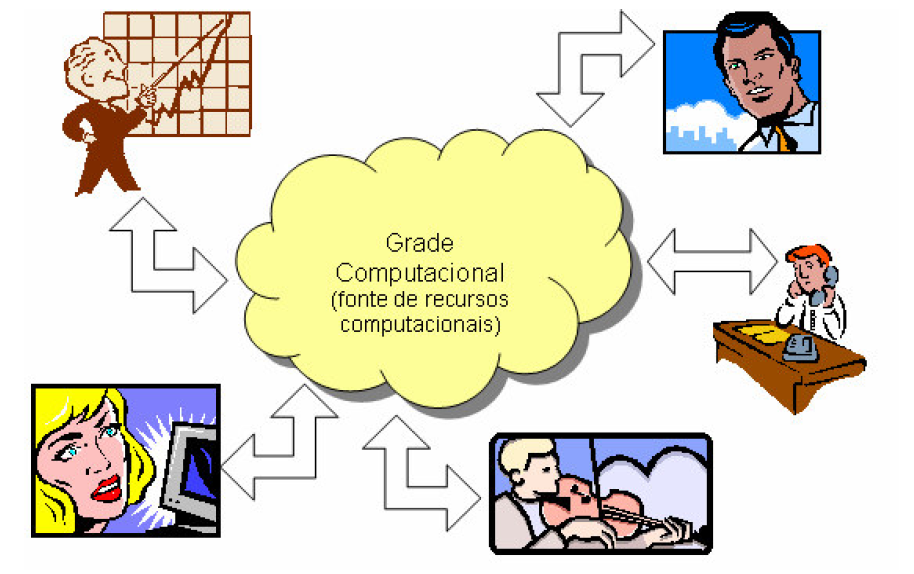
\includegraphics[width=0.6\textwidth]{figuras/grade-comp.png}
% 	% Caption centralizada
% % 	\captionsetup{justification=centering}
% 	% Caption e fonte 
% 	 \vspace{-0.2cm}
% 	\\\textbf{\footnotesize Fonte: \cite{cap-livro} }
% 	\label{fig:figura1}
% \end{figure}
% \vspace{-0.5cm}

% \subsection{\esp Inserção de tela de software}

% Nos casos de telas de \textit{software}, devem ser inseridas como figuras, e referenciadas no texto
% como na Figura \ref{fig:tela1}. Além disso, é necessário que seja citada no texto a empresa desenvolvedora.

% % Figura
% \begin{figure}[!ht]
% 	\centering	
% 	\caption[\hspace{0.1cm}Exemplo de tela de software.]{Exemplo de tela de software}
% 	  \vspace{-0.4cm}
% 	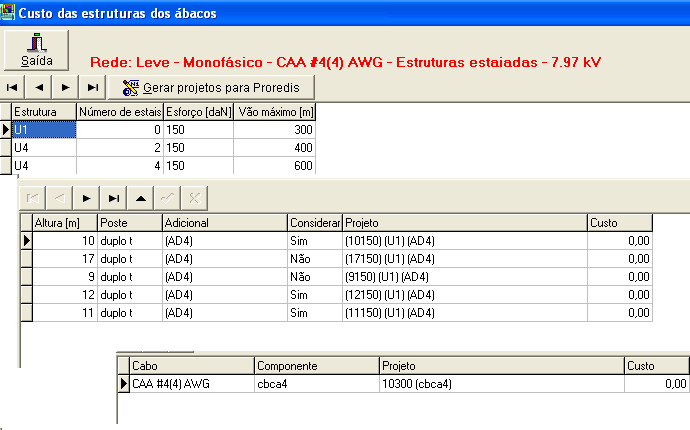
\includegraphics[width=.8\textwidth]{figuras/tela1.png}
% 	% Caption centralizada
% % 	\captionsetup{justification=centering}
% 	% Caption e fonte
% 	 \vspace{-0.3cm}
% 	\\\textbf{\footnotesize Fonte: \cite{tela1}}
% 	\label{fig:tela1}
% \end{figure}

% \subsection{\esp Inserção de gráficos e mapas}

% O gráfico é um tipo de ilustração que deve conter todos os elementos citados e também a descrição de seu título
% diferenciando-o das figuras da mesma forma que no Gráfico 1. 

% \begin{center}
% 	\centering	
%  	\textbf{Gráfico 1 - Exemplo de um gráfico} \\
% %  	  \vspace{0.cm}
% 	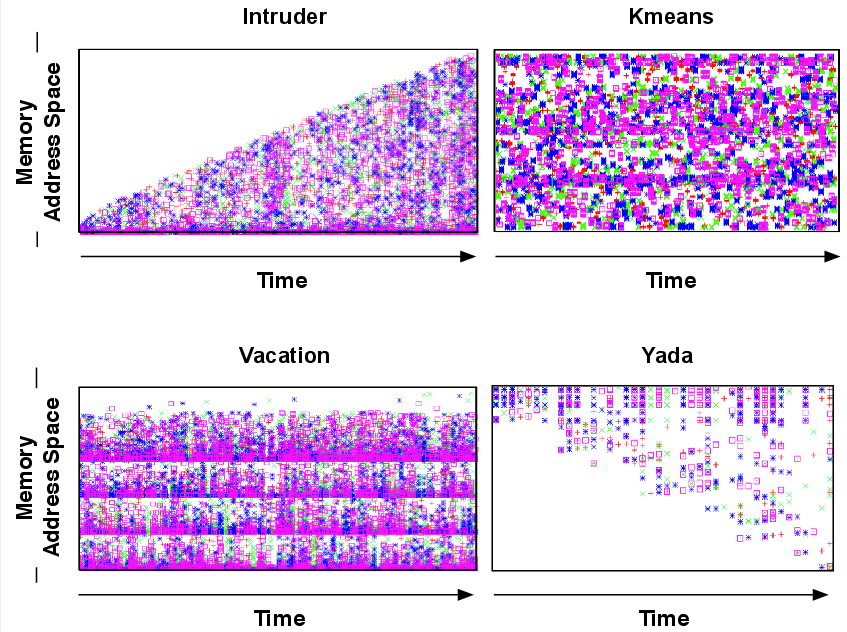
\includegraphics[width=0.7\textwidth]{figuras/access.png}
% 	% Caption centralizada
% % 	\captionsetup{justification=centering}
% 	% Caption e fonte
% 	 \vspace{-0.3cm}
% 	\\\textbf{\footnotesize Fonte: \cite{tese}}
% 	\label{grafico1}
% \end{center}

% A mesma regra se aplica para mapas, que devem ser adicionados seguindo as regras de apresentação já mostradas. No caso específico,
% o título e a numeração, também como os gráficos, devem começar do numeral ``1'' depois da marcação ``Mapa'' seguido do nome do elemento.
% Exemplo: \textbf{Mapa 1 - Exemplo de um Mapa}.

%  \subsection{\esp Tabelas}

% As tabelas devem ser abertas nas laterais, com espaços verticais separando
% as colunas e sem espaços horizontais, exceto na
% separação do cabeçalho. Um exemplo é a Tabela \ref{tab:tabela1}. 

% % Tabela
% \begin{table}[htb]
% 	\centering
% 	\caption{\hspace{0.1cm} Exemplo de uma tabela}
% 	\vspace{-0.3cm} % espaço entre titulo e tabela
% 	\label{tab:tabela1}
% 	% Conteúdo da tabela
% 	\begin{tabular}{l|c|c}
%   \hline
%     \textbf{Imagem}	& \textbf{transferência} & \textbf{tempo} \\
%     \hline
%      estação 1	& 7,72 MB/s &  1:22:18 \\
%      estação 2	& 7,72 MB/s &  1:22:17 \\
%      estação 3	& 7,59 MB/s & 1:24:25 \\
%      estação 4  & 7,53 MB/s & 1:43:27 \\
%      estação 5	& 6,14 MB/s  &  1:24:41 \\
%      estação 6  &  7,50 MB/s & 1:23:53 \\
%      estação 7  & 7,58 MB/s  &  1:24:02 \\
%      estação 8  & 7,8 MB/s  &  1:29:06 \\
%      estação 9  & 7,9 MB/s  &  1:30:05 \\
%      estação 10 & 8,0 MB/s  &  1:32:03 \\
%      \hline
%  \end{tabular}
%  	\vspace{.1cm}  %espaço entre tabela e fonte
% 	\small
% 	% Fonte
% 	{\footnotesize\\ \textbf{Fonte: \cite{monog-fabio}}}
% \end{table}

% \subsection{\esp Quadros}

% Os quadros diferem das tabelas por apresentarem dados textuais.
% Esses dados podem ser esquemáticos, comparativos ou descritivos.

%    \begin{center}
%           \centering
%        	\textbf{Quadro 1 - Bandas/Artistas de Rock e outros}\\
% % 	\vspace{-0.3cm} % espaço entre titulo e tabela
%         \label{quadro1}
% 	\begin{tabular}{|c|c|c|c|} \hline
% 	\multicolumn{4}{|c|}{\textbf{Bandas ou Artigas de Rock e outros}} 	  \\ 
% 		\hline \textbf{	Progressivo} & Pink Floyd & Jethro Tull	& Yesterday \\ 
% 		 \hline \textbf{ Metal}  & Metallica & Iron Maidam & Black Sabath \\ 
% 		\hline \textbf{	Arena Rock} & Led Zeppelin & The Rolling Stones & Beatles \\ 
% 		\hline \textbf{ Punk} & Ramones & Black Flag & NOFX	\\ 
% 		\hline \textbf{	Nacional} & Ira & Engenheiros & Vinil	\\ 
% 		\hline \textbf{	S.J.E.} & Apolo XI & Invasão 7 & Por do Sol \\ 
% 		\hline \textbf{	Grunge} & Nirvana & Pear Jam & Alice in Chains	\\ 
% 		\hline \textbf{	Rock Folk} & Bod Dylan & The Byrds &  The Mamas \& the Papas \\
% 		\hline \textbf{	Blues} & B.B. King & Albert Colins & Mady Wathers \\ 
% 		\hline \textbf{	New Wave} & The Police & The Pretenders, &  Duran Duran\\ 
%  		\hline \textbf{	Rock Folk} & Bod Dylan & The Byrds &  The Mamas \& the Papas \\
%  		\hline \textbf{	Rock alternativo} & R.E.M.& Hüsker Dü & Big Black\\ 
 		
% 		\hline
% 	\end{tabular}
% 	\vspace{0.1cm} 
% 	{\footnotesize\\ \textbf{Fonte: Dados da pesquisa}}
%    \end{center}

% Para gráficos, quadros e tabelas, cujos dados foram extraídos da própria pesquisa, 
%  usar a expressão: Dados da pesquisa. Ver exemplo no Quadro 1.
   

% \subsection{\esp Inserção de algoritmos}

% Para inserir um algoritmo, utilizar o exemplo do Algoritmo  \ref{alg:rnagenerica}.
% Todos os algoritmos devem ser inseridos como figura, indicada por nome e  fonte. Caso 
% forem de própria autoria, isso deverá ser mencionado na fonte, como elaboração feita pelos autores.

% % algoritmo
% % \begin{figure}[ht]
% \begin{center}	
% 	% Arquivo da figura
% % 	\caption[\hspace{0.1cm} Texto da figuras.]{Algorítmo CAC RD Neural}
%          \textbf{Algoritmo 1 -  CAC RD Neural}
% 	\vspace{-0.3cm}
% \begin{minipage}[ht]{13cm}
% \begin{algorithm}[H]
%   \footnotesize
%   \caption{CAC-RD Neural}
%   \label{alg:rnagenerica}
%   \begin{algorithmic}[1]
%       \STATE \textbf{Entrada:} Requisição da chamada
%     \STATE \textbf{Saída:} Aceitação ou bloqueio da solicitação
    
%     \STATE Preenche o vetor de $attributes.size+1$ atributos com os valores dos atributos, sendo a primeira posição do vetor preenchida com o valor 1
% 		\STATE $hidden\_layer\_size =  attributes.size*2+1;$

%     \FOR{$i$ = 1 to $attributes.size+1$}
%     	\STATE \textbf{normalizar}($Entrada_i$)
%     \ENDFOR

% 		\STATE $double [] net = new double [hidden\_layer\_size];$
%     \STATE $net = hidden\_layer\_weights * attributes;$
%    	\FOR{$i$ = 0 to hidden\_layer\_size}
% 			\STATE $net [i] = 1.0 / (1.0 + exp((-1.0)*net[i]));$
% 		\ENDFOR

% 		\STATE $double [] ipVector = new double [hidden\_layer\_size+1];$
%     \STATE $ipVector [0] = 1.0;$
%    	\FOR{$i$ = 1 to $hidden\_layer\_size+1$}
% 			\STATE $ipVector [i] = net [i-1];$
% 		\ENDFOR
		
% 		\STATE $output = output\_layer\_weights *  ipVector;$
%     \STATE output = \textbf{desnormalizar}(Saída)
%     \STATE \textbf{net\_update} (requisition);
    
%     \STATE \textbf{Retorna} output; FIM
%   \end{algorithmic}
% \end{algorithm}
% % \vspace{-0.3cm} % espaço entre algoritmo e fonte

% \small \centering \textbf{\footnotesize Fonte: \cite{mestrado}.}
% \end{minipage}
% \end{center}
% % \end{figure}

% Para ilustrações criadas ou adaptadas a partir de outras ilustrações, usar as expressões: 
% “Adaptado de...” ou “Criado pelo autor`` com dados extraídos de \ldots
   
   
\section{\esp CITAÇÕES}


Referências deverão ser adicionadas no arquivo \textit{bibliografia.bib}. Cada referência deverá ser adicionada conforme o padrão de normalização da PUC, 
o qual poderá ser consultado na página da biblioteca da PUC Minas \cite{manualpuc}. Todas as publicações citadas no texto deverão ter correspondente nas referências, 
e as indicações de autoria da citação e do ano deverão ser idênticas aos dados expostos.


\subsection{\esp Citação livre ou indireta}

Quando se reproduzir ideias, sem transcrever as palavras do autor, a indicação da página é opcional. Exemplos desse tipo de citação:
\begin{enumerate} 
 \item [a)] Citação com um autor \cite{knuth}. 
 \item [b)] Citação de artigos em revistas com dois autores \cite{artigo01}.
  \item [c)] Trabalho em congresso com três autores \cite{dovzan:01}.
 \item [d)] Trabalhos com mais de três autores \cite{cap-livro}.
 \item [e)] Dois autores em duas obras distintas \cite{knuth,groupp}.
 \item [d)] Trabalhos distintos com vários autores \cite{congresso,cap-livro}.
 
\end{enumerate}

\subsection{\esp Citação direta ou textual}

Transcrição literal de textos de outros autores. Nesse caso, deverão ser especificadas as páginas consultadas. 
Se desejar, poderão ser grafadas em itálico para melhor visualização.

\subsubsection{\esp Textual Curtas}

Quando curtas (até 3 linhas) serão inseridas na sequência normal do texto, entre aspas com as mesma formatação.

\subsubsection{\esp Textual Longas}

Citações longas (mais de 3 linhas) deverão constituir um parágrafo independente, recuado a 4 cm da margem esquerda, 
com letra tamanho 10 e digitado em espaço simples, sem aspas.
\begin{citacaodireta}
Hegel chama trabalho à forma específica da satisfação das necessidades, que
distingue da natureza o espírito existente. Assim como a linguagem infringe
a imposição da intuição e ordena o caos das múltiplas sensações em coisas
identificáveis, assim o trabalho infringe a imposição do \hspace{0.1cm}desejo \hspace{0.1cm}imediato \hspace{0.1cm}e
suspende, por assim dizer, o processo de satisfação das necessidades.
\cite[25]{habermas}.
\end{citacaodireta}


% Artigo \cite{whatershed:01}

\subsubsection{\esp Textual de outros idiomas (Tradução)}

\begin{citacaodireta} 
Um \textit{cluster} é um computador paralelo construído de componentes e processos de \textit{software} (tal como sistema de \textit{software}). 
Um \textit{cluster} é formado de nós, cada um contendo um ou mais processadores, memória que é compartilhada por todos os processadores do nodo 
(somente eles), e dispositivos periféricos adicionais (tais como discos), conectados pela rede e que permitem tráfego de dados entre os nós...
\cite[p. 10, tradução nossa]{groupp}\footnote {  … a cluster is a parallel computer that is constructed of commodity  componets and runs 
(as its system software) commodity software. A cluster is made of nodes, each conteining one or more processors, memory that is  shared 
by all of the processors in (and only on) the node, and addtional peripheral devices (surch as disks),
 connected by network that allows data to move between the nodes}.
\end{citacaodireta}
 
\subsection{\esp Exemplos de citações} 

Alguns exemplos de citações mais utilizadas e/ou que geram algumas dúvidas. É válido observar que não citaremos
todas as possibilidades de citações da norma da PUC Minas, sendo assim é de extrema relevância que se consulte 
o documento no site da Biblioteca da PUC Minas para maiores esclarecimentos acerca de citações \cite{manualpuc}.

\subsubsection{\esp Citação de monografia, dissertação e tese}

Exemplo de citação de monografia de curso de graduação ou especialização pode ser vista em \citeonline{monog-fabio}.
Exemplo de dissertação de mestrado é referida como \citeonline{mestrado}.

Para o caso de doutorado é citado da seguinte forma, Góes (\citeyear{tese}). Nesse exemplo é válido observar a forma
como está escrito no documento \LaTeX, pois citações que compreendem no texto o nome do autor como sua parte, necessitam 
do parâmetro \verb$\citeonline{}$. 

\subsubsection{\esp Livros e partes de livros}

Exemplo de capítulo de livro fica conforme este exemplo \cite{cap-livro}.

Para livros citados no corpo do texto e com duas citações juntas, ver os exemplos \citeonline{knuth,groupp}.
Caso essa citação não fizesse parte do texto será referencia dessa forma \cite{knuth,groupp}.

Citações institucionais ou documentos técnicos de alguma entidade devem ser citados desta forma \cite{pmbok}.

\subsubsection{\esp Tela de software}

Para  citar a tela de um \textit{software} faça da seguinte forma, \citeonline{tela1}.

\subsubsection{\esp Citações da Biblia Sagrada}

A Bíblia está dividida em duas grandes partes: O Antigo Testamento e o Novo Testamento, divididos em livros, capítulos e versículos. 
Portanto, a citação de partes da Bíblia deve apresentar o título do livro de forma abreviada ou por extenso, o número do capítulo e o número do versículo.

\begin{citacaodireta}
Moisés estendeu a mão sobre o mar. Com um forte \hspace{-0.1cm} vento \hspace{0.1cm} leste a \hspace{0.1cm}sobrar a
noite toda, o Senhor repeliu o mar e o pôs a seco. As águas se fenderam e
os filhos de Israel entraram no meio do mar a pé enxuto, enquanto as águas
formavam uma muralha à direita e à esquerda deles (\citeauthor{biblia} 14,21).
\end{citacaodireta}

\subsection{\esp Conclusão}

Discussão dos resultados obtidos na pesquisa. É onde se colocam as observações do autor. 
Poderá também apresentar sugestões de novas linhas de estudo.

A conclusão deve estar de acordo com os objetivos do trabalho.

A conclusão não deve apresentar citações ou interpretações de outros autores.

\subsection{\esp Trabalhos futuros}

Sugestões de estudos posteriores são ser adicionados subseção deste capítulo de conclusão.